%\title{Automatic Generation of Ceph Performance Reports}
%\author{Jos\'e J Palacios P\'erez}
%\maketitle
\documentclass[titlepage]{report}
\usepackage{graphicx,booktabs,array}
\usepackage[a4paper, total={7in, 10.5in}]{geometry}
\usepackage{hyperref}
\hypersetup{linkcolor=blue,citecolor=blue,filecolor=blue,urlcolor=blue} % blue links, for printed output
\usepackage[T1]{fontenc}
%\usepackage[printwatermark]{xwatermark}
\usepackage{draftwatermark}

\usepackage{xcolor}
\usepackage{fancyhdr}
%\newwatermark[allpages,color=red!50,angle=45,scale=3,xpos=0,ypos=0]{DRAFT}
%\newwatermark[allpages,angle=45,scale=3,xpos=0,ypos=0]{DRAFT}

\makeatletter
\def\@makechapterhead#1{%
  {\parindent \z@ \raggedright \normalfont
    \ifnum \c@secnumdepth >\m@ne
        \huge\bfseries \thechapter.\ % <-- Chapter # (without "Chapter")
    \fi
    \interlinepenalty\@M
    #1\par\nobreak% <------------------ Chapter title
    \vskip 20\p@% <------------------ Space between chapter title and first paragraph
  }}
\makeatother

% macro to insert a figure within a table
\newcommand{\addpic}[1]{\includegraphics[width=0.45\textwidth]{#1}}
\newcolumntype{C}{>{\centering\arraybackslash}m{0.45\textwidth}}
\makeatletter
\newcolumntype{V}[1]{>{\topsep=0pt\@minipagetrue}p{#1}<{\vspace{-\baselineskip}}}
\makeatother
\newcommand{\command}[1]{\texttt{\string#1}}

% These macros should be worked out by the report gneration script:
% \input{definitions.tex}
% \newcommand{\sea_folderrr}{../data/osd_1_28reactor_28fio_rc_seastore/}
% \newcommand{\sea_folderrw}{../data/osd_1_28reactor_28fio_cmp_sea_classic/sea_1osd_28reactor_32fio_bal_osd_rc_1procs_randwrite_d/}
% \newcommand{\sea_foldersr}{../data/osd_1_28reactor_28fio_cmp_sea_classic/sea_1osd_28reactor_32fio_bal_osd_rc_1procs_seqread_d/}
% \newcommand{\sea_foldersw}{../data/osd_1_28reactor_28fio_cmp_sea_classic/sea_1osd_28reactor_32fio_bal_osd_rc_1procs_seqwrite_d/}
%
% \newcommand{\cla_folderrr}{../data/osd_1_56cpu_28fio_rc_classic/classic_1osd_32fio_rc_1procs_randread.zip}
% \newcommand{\cla_folderrw}{../data/osd_1_56cpu_28fio_rc_classic/classic_1osd_32fio_rc_1procs_randwrite.zip}
% \newcommand{\cla_foldersr}{../data/osd_1_56cpu_28fio_rc_classic/classic_1osd_32fio_rc_1procs_seqread.zip}
% \newcommand{\cla_foldersw}{../data/osd_1_56cpu_28fio_rc_classic/classic_1osd_32fio_rc_1procs_seqwrite.zip}
% %\newcommand{\folder}{../_sea_1osd_28reactor_32fio_bal_osd_rc_1procs_randread_d/}

%\makeatletter
%\def\input@path{{/path/to/folder/}}
%or: \def\input@path{{/path/to/folder/}{/path/to/other/folder/}}
%\makeatother

\begin{document}

%% Set the page style to "fancy"...
% \pagestyle{fancy}
% %... then configure it.
% \fancyhead{} % clear all header fields
% \fancyhead[RO,LE]{\textbf{(DRAFT)}}
% \fancyfoot{} % clear all footer fields
% \fancyfoot[LE,RO]{\thepage} % page number in "outer" position
% \fancyfoot[CO,CE]{\textbf{(DRAFT)}}
%
\title{\textbf{Crimson vs. Async Messenger Performance Comparison} -- progress report}
\author{Jos\'e Juan Palacios P\'erez\\Ceph IBM,\\Manchester UK}
\date{\today}

\begin{titlepage}
 \begin{minipage}{\textwidth}
   \begin{center}
      
\includegraphics[width=0.3\textwidth]{ceph_362px.png}
      %\vspace*{1cm}
      \maketitle
      %\vspace*{1cm}
   \end{center}
   \begin{abstract} 
  In this brief report we summarise the performance results for the comparison
  between the Crimson SeaStore using the following configurations:
  \begin{itemize}
    \item single Seastar reactor per physical core: up to 28 reactors, single NUMA socket,
    \item dual Seastar reactor per physical core: up to 56 reactors, single NUMA socket.
    \item We used the same ceph dev build from main branch (hash 6aab5c07ae) for both.
    \item We only used the balanced OSD algorithm.
  \end{itemize}
Our preliminary conclusions:
  \begin{itemize}
    \item The performance of the Crimson SeaStore using the dual Seastar
	reactor per physical core achieves better performance across the four typical workloads. 
  This suggest that Seastar is HT-friendly in the sense that reactors don't
      seem to interfere each other use of the physical CPU.
  \end{itemize}
\end{abstract}


   %\Huge
   %\textbf{Automatic Generation of Ceph Performance Reports}
   \vspace{0.5cm}
           %\LARGE
   %{\small This report was mechanically generated by the toolkit in \url{https://github.com/perezjosibm/ceph-aprg}.}
   \vfill
   %\vspace{0.8cm}
  \end{minipage}
\end{titlepage}
\tableofcontents
%\listoftables


%\input{01-latency-target}
%\graphicspath{ {./sea_vs_blue_f781c5/} }
\graphicspath{ {../figures/} }

\chapter{Seastore performance scaling}

In this Chapter we show the performance scaling of Seastore (build 87d2085) on longer
duration test sets, producing response latency curves. 

\begin{enumerate}
  \item We used a single OSD, running within a single NUMA socket, we only increased the number of reactors as indicated.
  \item We used the balanced OSD algorithm.
  \item We used 32 RBD images, each of 2GB size, four jobs per image. All FIO processes were pinned to the other NUMA socket, so that the OSD processes were not affected by the FIO processes.
  \item We disabled RBD coalescing so the sequential workloads would not be affected by the coalescing algorithm.
\end{enumerate}
%\pagebreak
\section{Random read 4k}

\begin{figure}[!ht]
  \centering
  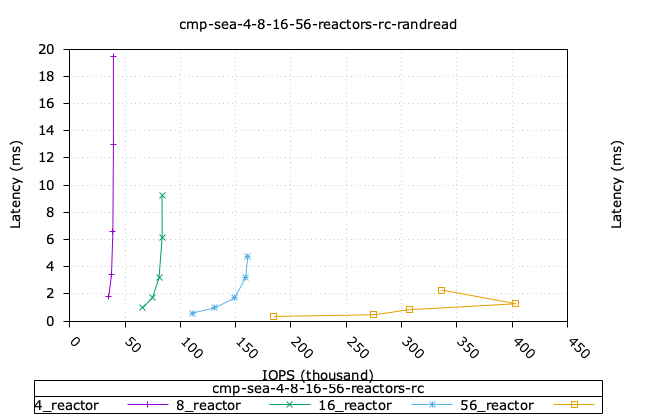
\includegraphics[width=0.9\textwidth]{cmp_sea_4_8_16_56_reactors_rc_randread_iops_vs_lat.png}
  \caption{Response latency curves, IOPs vs. Latency. Each curve is for a different number of reactors, 4, 8, 16 and 56. Each datra point corresponds to an increasing IO depth, from 1 2 4 8 16 24 32 40 52 to 64. If the latency is higher than 1 sec, the data point is not shown. The x-axis is the IOPs, the y-axis is the latency in milliseconds.}
\end{figure}

% utilisation:OSD
% \begin{figure}[h]
%   \centering
%   \begin{minipage}{.5\textwidth}
%   \centering
%     \includegraphics[width=\textwidth]{classic_vs_seastore_1osd_32fio_randread_iops_vs_lat_osd_cpu.png}
%     %\caption{4k random read}
%      %\label{figure:sea_4k_randread}
%   \end{minipage}%
%   \begin{minipage}{.5\textwidth}
%   \centering
%     \includegraphics[width=\textwidth]{classic_vs_seastore_1osd_32fio_randread_iops_vs_lat_osd_mem.png}
%     %\caption{System CPU utilisation}
%     %\label{figure:sea_4k_randwrite}
%   \end{minipage}%
% \end{figure}
%
%In the Tables below we show the performance figures for the workloads above.
% Table showing the figures for this workload
%pagebreak

\section{Random write 4k}

\begin{figure}[ht!]
  \centering
  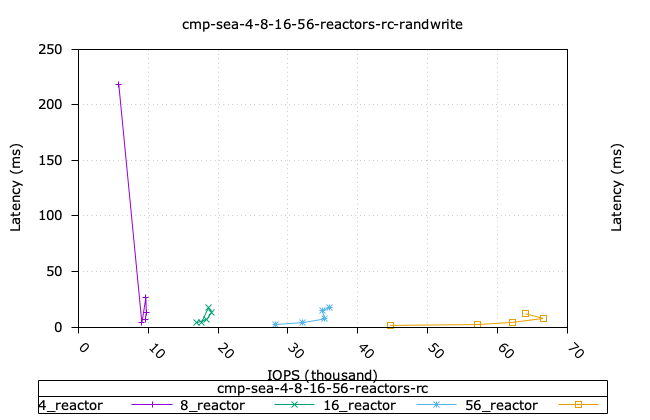
\includegraphics[width=0.9\textwidth]{cmp_sea_4_8_16_56_reactors_rc_randwrite_iops_vs_lat.png}
\end{figure}

% utilisation:OSD
% \begin{figure}[h]
%   \centering
%   \begin{minipage}{.5\textwidth}
%   \centering
%     \includegraphics[width=\textwidth]{classic_vs_seastore_1osd_32fio_randwrite_iops_vs_lat_osd_cpu.png}
%     %\caption{4k random write}
%      %\label{figure:sea_4k_randwrite}
%   \end{minipage}%
%   \begin{minipage}{.5\textwidth}
%   \centering
%     \includegraphics[width=\textwidth]{classic_vs_seastore_1osd_32fio_randwrite_iops_vs_lat_osd_mem.png}
%     %\caption{System CPU utilisation}
%     %\label{figure:sea_4k_randwrite}
%   \end{minipage}%
% \end{figure}
\newpage
\pagebreak

\section{Sequential read 64k}

\begin{figure}[ht]
  \centering
  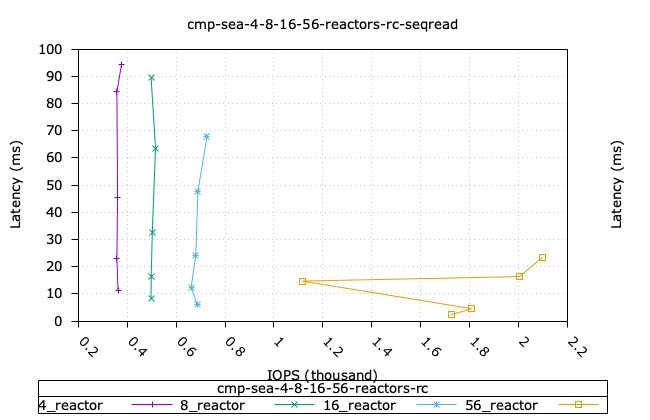
\includegraphics[width=0.9\textwidth]{cmp_sea_4_8_16_56_reactors_rc_seqread_iops_vs_lat.png}
  %\caption{Response latency curves, IOPs vs. Latency}
\end{figure}

% utilisation:OSD
% \begin{figure}[h]
%   \centering
%   \begin{minipage}{.5\textwidth}
%   \centering
%     \includegraphics[width=\textwidth]{classic_vs_seastore_1osd_32fio_seqread_iops_vs_lat_osd_cpu.png}
%     %\caption{4k random write}
%      %\label{figure:sea_4k_seqread}
%   \end{minipage}%
%   \begin{minipage}{.5\textwidth}
%   \centering
%     \includegraphics[width=\textwidth]{classic_vs_seastore_1osd_32fio_seqread_iops_vs_lat_osd_mem.png}
%     %\caption{System CPU utilisation}
%     %\label{figure:sea_4k_seqread}
%   \end{minipage}%
% \end{figure}
%
\newpage
\pagebreak

\section{Sequential write 64k}

\begin{figure}[ht]
  \centering
  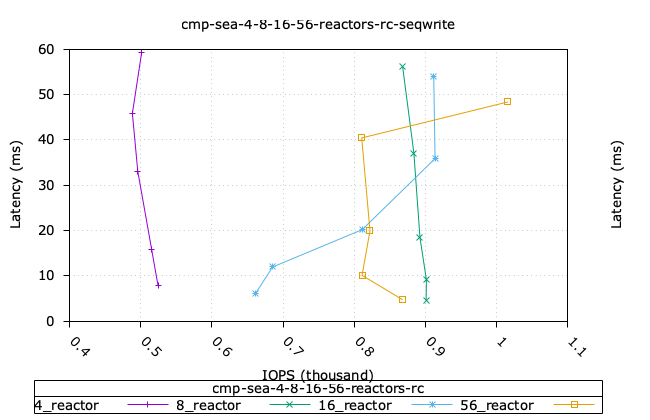
\includegraphics[width=0.9\textwidth]{cmp_sea_4_8_16_56_reactors_rc_seqwrite_iops_vs_lat.png}
  %\caption{Response latency curves, IOPs vs. Latency}
\end{figure}

% % utilisation:OSD
% \begin{figure}[h]
%   \centering
%   \begin{minipage}{.5\textwidth}
%   \centering
%     \includegraphics[width=\textwidth]{classic_vs_seastore_1osd_32fio_seqwrite_iops_vs_lat_osd_cpu.png}
%     %\caption{4k random write}
%      %\label{figure:sea_4k_seqwrite}
%   \end{minipage}%
%   \begin{minipage}{.5\textwidth}
%   \centering
%     \includegraphics[width=\textwidth]{classic_vs_seastore_1osd_32fio_seqwrite_iops_vs_lat_osd_mem.png}
%     %\caption{System CPU utilisation}
%     %\label{figure:sea_4k_seqwrite}
%   \end{minipage}%
% \end{figure}
%
%\newpage



\clearpage

\appendix
%\input{configuration}
%\input{estimation}

\end{document}
%%%%%%%%%%%%%%%%%%%%%%%%%%%%%%

